\documentclass[dvipsnames,tikz]{standalone}
\usepackage{amsmath}
\usepackage{arevmath}
\usepackage{xcolor}
\usepackage{tikz}
\usetikzlibrary{calc}
\usetikzlibrary{decorations.pathreplacing,calligraphy,3d}
\usepackage{tikz-3dplot} 

\tikzset{main/.style={thick, circle, color=black}}

\usetikzlibrary{decorations.pathmorphing,patterns}

\makeatletter

\pgfdeclaredecoration{penciline}{initial}{
	\state{initial}[width=+\pgfdecoratedinputsegmentremainingdistance,auto corner on length=1mm,]{
		\pgfpathcurveto%
		{% From
			\pgfqpoint{\pgfdecoratedinputsegmentremainingdistance}
			{\pgfdecorationsegmentamplitude}
		}
		{%  Control 1
			\pgfmathrand
			\pgfpointadd{\pgfqpoint{\pgfdecoratedinputsegmentremainingdistance}{0pt}}
			{\pgfqpoint{-\pgfdecorationsegmentaspect\pgfdecoratedinputsegmentremainingdistance}%
				{\pgfmathresult\pgfdecorationsegmentamplitude}
			}
		}
		{%TO 
			\pgfpointadd{\pgfpointdecoratedinputsegmentlast}{\pgfpoint{1pt}{1pt}}
		}
	}
	\state{final}{}
}
\makeatother

\begin{document}
	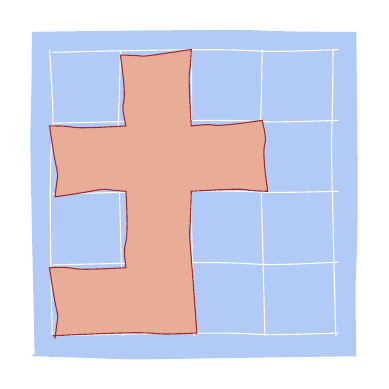
\begin{tikzpicture}[outer sep=0.05cm,node distance=0.8cm,decoration=penciline, scale=0.9]
		\fill[decorate, CornflowerBlue, semitransparent] (-0.25,-0.25) rectangle (4.25,4.25);
		\draw[decorate,white] (0,0) grid[step=1cm] (4,4);
		\draw[decorate, color=Brown, fill=BrickRed!30] (0,0) -- (2,0) -- (2,2) -- (3,2) -- (3,3) -- (2,3) -- (2,4) -- (1,4) -- (1,3) -- (0,3) -- (0,2) -- (1,2) -- (1,1)-- (0,1) -- cycle;
	\end{tikzpicture}

\end{document}